\chapter[AGES I --- “VÍTIMAS DE CRIME”]{AGES I --- “VÍTIMAS DE CRIME”}

Esta seção busca apresentar a passagem do aluno como AGES I pelo projeto Vítimas de Crime. Seguem descritos os artefatos entregues, a atuação ao longo das sprints e os pontos de melhoria identificados pelo aluno.

\section[Introdução]{Introdução}

O projeto Vítimas de Crime teve como princípio garantir o direito à informação para vítimas de crime no estado do Rio Grande do Sul. A principal stakeholder do projeto era a promotora de justiça criminal de Viamão Dra. Márcia Vilanova.

Seu objetivo consistia no desenvolvimento de um aplicativo acessível às
vítimas, permitindo que estas alimentassem o sistema com provas e documentos de procedimentos criminais. Dessa forma, as informações seriam encaminhadas primeiro para a Polícia Civil e, posteriormente, para o Ministério Público, instruindo assim o processo. Especificamente, era vital garantir três pilares de direitos às vítimas: o Acesso à informação, a plena realização dos direitos e a devida proteção.

O primeiro pilar abrange esclarecimentos na plataforma virtual sobre o rito dos crimes comuns apenados com reclusão como roubo, furto, latrocínio ou estelionato, incluindo desde o registro de ocorrência policial até a conclusão do Inquérito Policial. Além disso, abrange leis especiais, como o estatuto do idoso e o estatuto da criança
e do adolescente.

O segundo pilar é dedicado ao exercício de direitos, envolvendo a prerrogativa de ser atendida, ouvida e a de buscar os órgãos de repressão do Estado. Este processo inclui fornecer informações detalhadas sobre contatos telefônicos e endereços, garantindo que as vítimas possam acessar de maneira efetiva e informada os recursos disponíveis as mesmas.

Por fim, o terceiro pilar visa buscar e garantir direitos de cidadania na rede municipal. Essa iniciativa aspira proporcionar atendimento médico, psiquiátrico e social para auxiliar na reestruturação da vida após o trauma causado pelo ilícito criminoso, incluindo considerações sobre mudanças de endereço, trabalho, escola, e outros aspectos relevantes para a reintegração plena da vítima na sociedade.

As datas de início e fim do projeto foram de 14/08/2023 a 20/11/2023 e contou com a orientação e suporte do prof. Dr. Daniel Callegari. A Figura 1 apresenta o time responsável pelo projeto.

\begin{figure}[H]
    \centering
    \small
    \caption{Time do projeto Vítimas de Crime}
    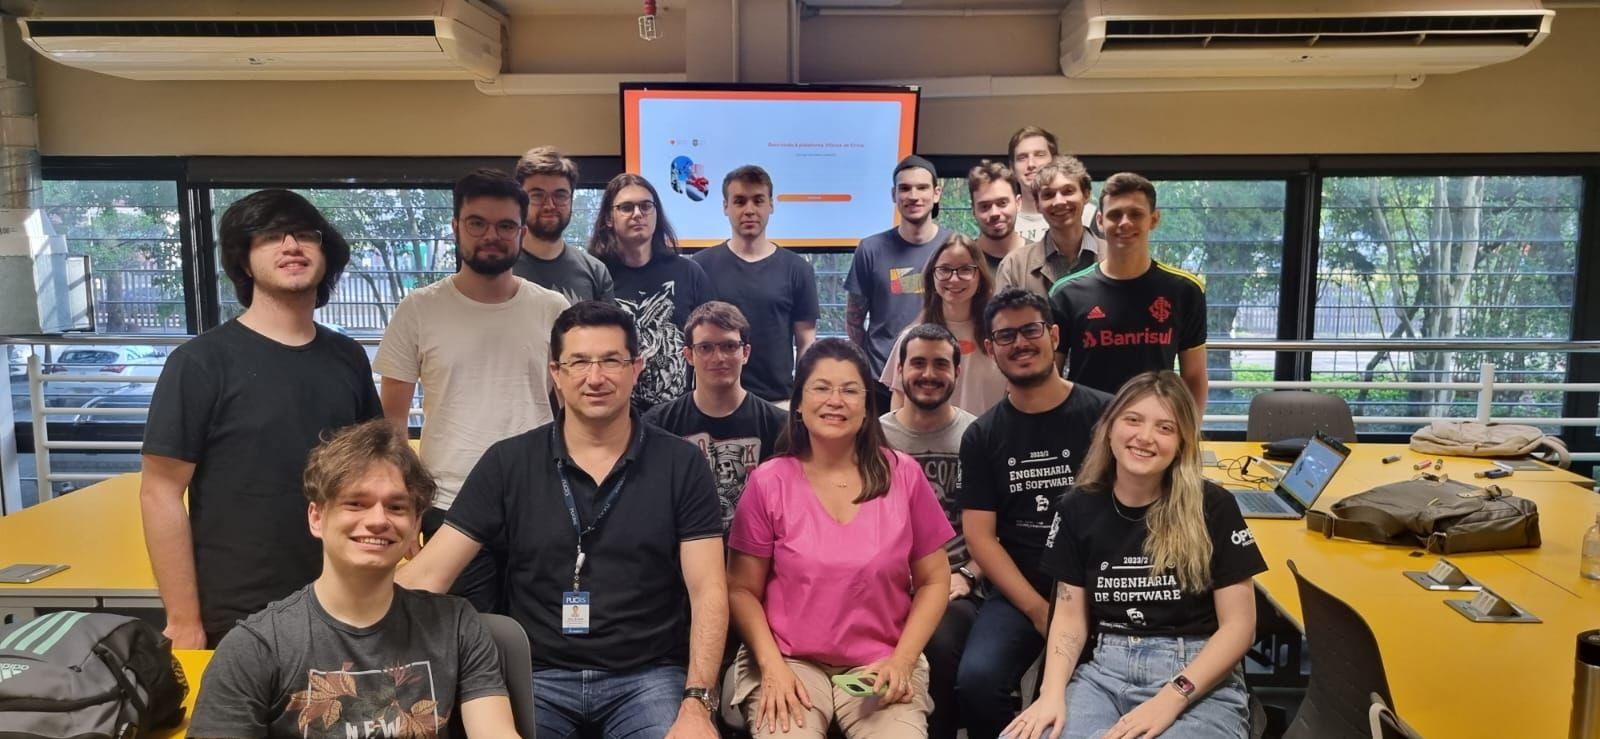
\includegraphics[width=1\linewidth]{conteudo//2 - ages I//conteudo//figures/figura1-time}
    Fonte: Autor
    \label{fig:projeto-time}
\end{figure}
\section[Desenvolvimento do Projeto]{Desenvolvimento do Projeto}
  Ao longo desta seção, são apresentados os artefatos desenvolvidos ao longo do semestre no qual se situou o projeto. Também estão descritas as etapas realizadas
  para as entregas destes artefatos, bem como ilustrações e seus respectivos links.

\subsection{Repositório do Código Fonte do Projeto}
  Inicialmente foram criados cinco repositórios para o projeto, sendo eles: “Wiki”, “App”, “Web”, “Auth” e “Api”. O repositório “Wiki” contava com a documentação do trabalho, contendo desde o fluxo de trabalho utilizado, arquitetura, \textit{desing/mockups} além de demais informações. “App” e “Web” contavam com o desenvolvimento do \textit{frontend} do projeto tanto para mobile quanto para web respectivamente. Já “Auth” e “Api” serviam para a lógica do \textit{backend} do projeto todo.
  
Ao longo do semestre mais dois repositórios foram criados. “Infrastructure” era
responsável pelo armazenamento de arquivos de configuração de CI/CD assim como
12
as configurações na nuvem. Por fim, “E2E Tests” foi criado como o repositório de
testes de sistema do projeto utilizando \textit{Selenium}. Todos os repositórios podem ser
encontrados em: https://tools.ages.pucrs.br/vitimas-de-crime.

\subsection{Banco de Dados Utilizado}
  A escolha feita para o projeto de acordo com os requisitos levantados foi de um
banco relacional. Ao decorrer do desenvolvimento e das apresentações para os
stakeholders, pequenas mudanças foram feitas nos diagramas. Ilustradas na Figura 2
e Figura 3 estão o diagrama de entidade-relacionamento e o esquema lógico final
respectivamente.

\begin{figure}[H]
    \centering
    \small
    \caption{Diagrama de entidade-relacionamento do banco de dados do projeto Vítimas de Crime}
    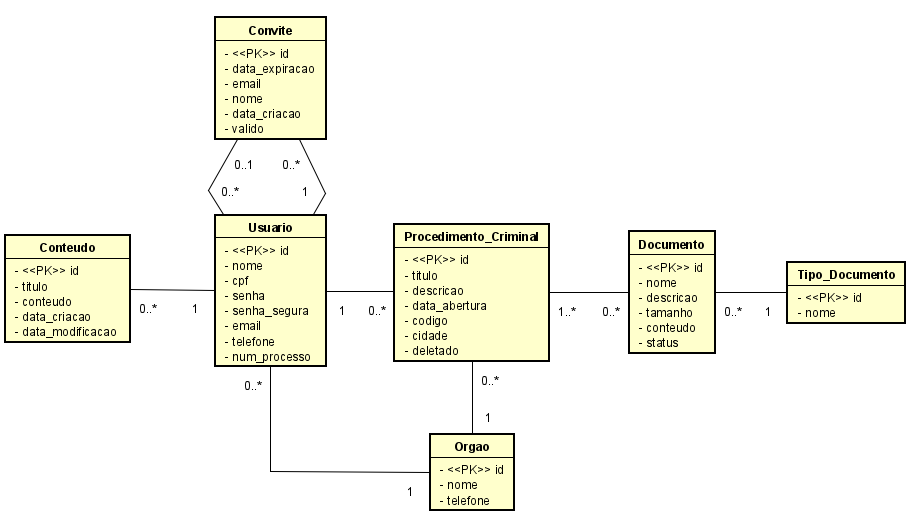
\includegraphics[width=1\linewidth]{conteudo//2 - ages I//conteudo//figures/figura2-esquema-bd}
    Fonte: \textit{Wiki} do projeto
    \label{fig:db-init}
\end{figure}

\begin{figure}[H]
    \centering
    \small
    \caption{Esquema lógico final do banco de dados do projeto Vítimas de Crime}
    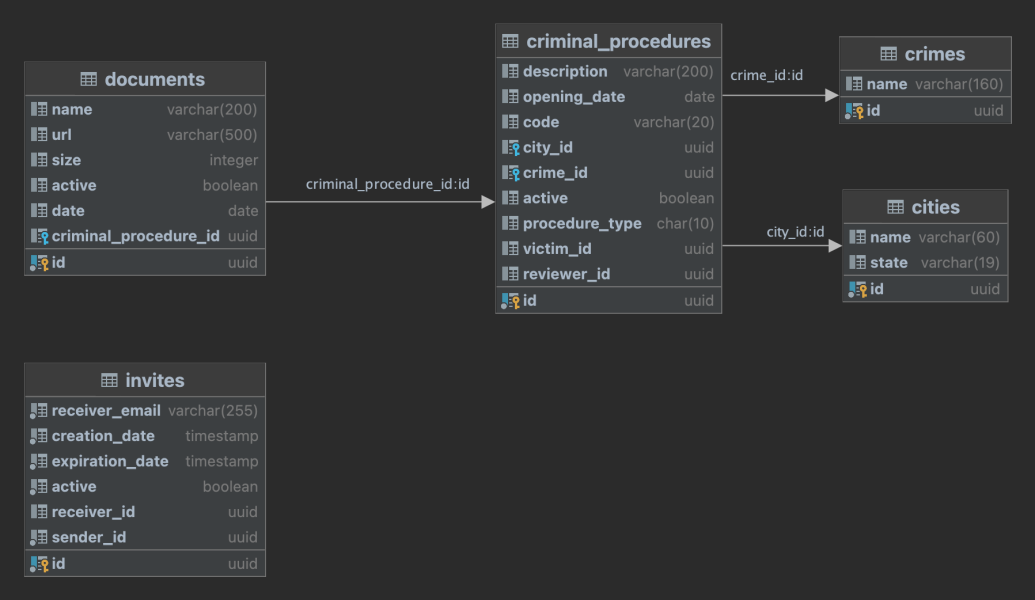
\includegraphics[width=1\linewidth]{conteudo//2 - ages I//conteudo//figures/figura3-logico-bd}
    Fonte: \textit{Wiki} do projeto
    \label{fig:db-schema}
\end{figure}

\subsection{Arquitetura Utilizada}
  A modelagem da arquitetura segue o design de cliente/servidor em camadas,
na qual os clientes requisitam serviços ou recursos e os servidores respondem,
fornecendo esses recursos, seguindo um paradigma de comunicação estabelecido. A
Figura 4 ilustra cada componente que representa o modelo idealizado.


\begin{figure}[H]
    \centering
    \small
    \caption{Diagrama dos componentes da arquitetura do projeto Vítimas de Crime}
    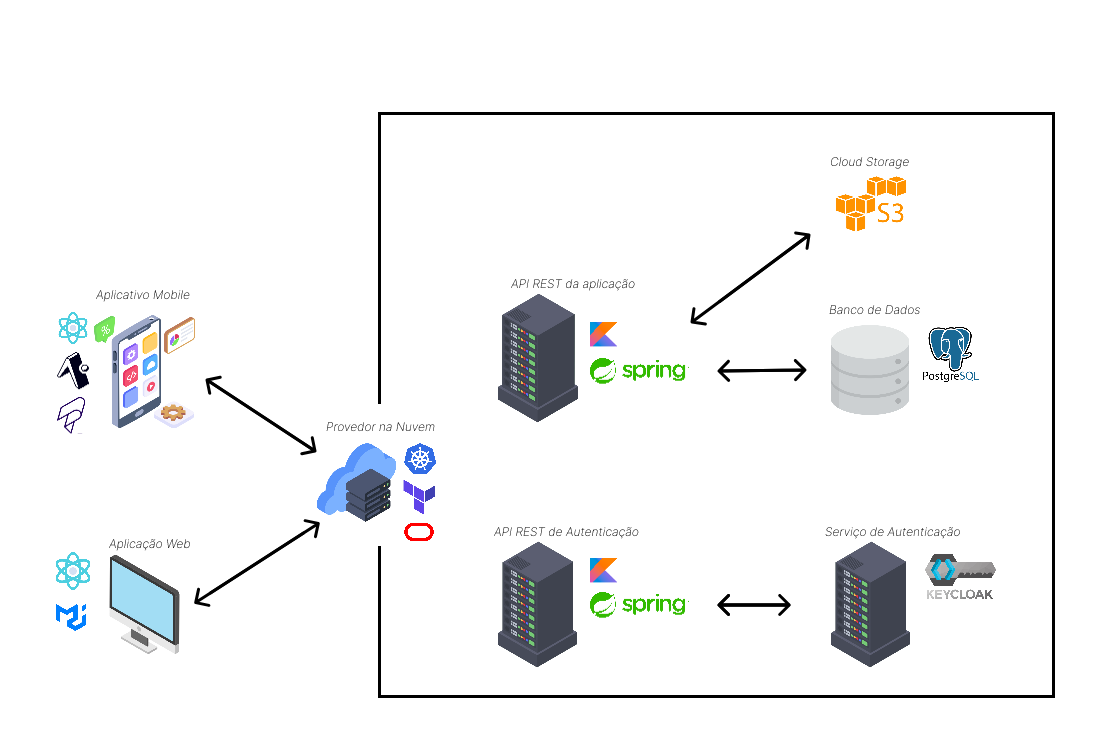
\includegraphics[width=1\linewidth]{conteudo//2 - ages I//conteudo//figures/figura4-diag-arq}
    Fonte: \textit{Wiki} do projeto
    \label{fig:components-arch}
\end{figure}

Na parte do servidor, as APIs REST da aplicação e de autenticação conversam
com seus respectivos recursos como o próprio banco de dados e o serviço de
autenticação. Os nossos clientes são os dispositivos mobile e web fazendo as
requisições a esse mesmo servidor.

\subsection{Protótipos das Telas Desenvolvidas}
  Os primeiros mockups do aplicativo mobile foram idealizados utilizando a
ferramenta Figma. Estes protótipos são apresentados nas Figuras 5, 6 e 7.

\begin{figure}[H]
    \centering
    \small
    \caption{Protótipo das telas mobile de cadastro do projeto Vítimas de Crime}
    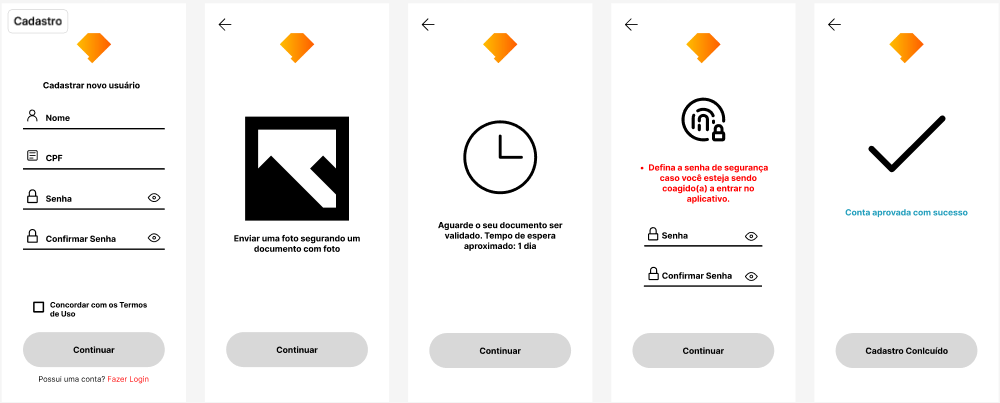
\includegraphics[width=1\linewidth]{conteudo//2 - ages I//conteudo//figures/figura5-prototipo-telas}
    Fonte: Figma do projeto
    \label{fig:mobile-signup}
\end{figure}

\begin{figure}[H]
    \centering
    \small
    \caption{Protótipo das telas mobile de envio de documentos do projeto Vítimas de Crime}
    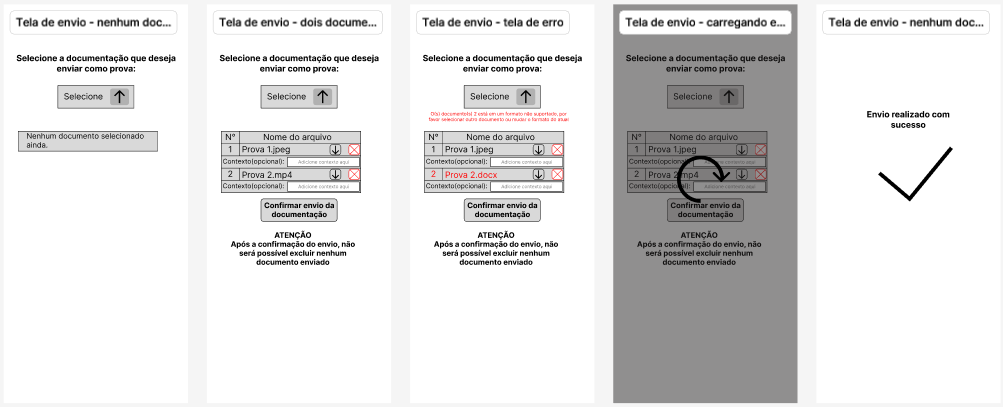
\includegraphics[width=1\linewidth]{conteudo//2 - ages I//conteudo//figures/figura6-prototipo-telas-resto}
    Fonte: Figma do projeto
    \label{fig:mobile-docs}
\end{figure}

\begin{figure}[H]
    \centering
    \small
    \caption{Protótipo das telas mobile de visualização de documentos do projeto Vítimas de Crime}
    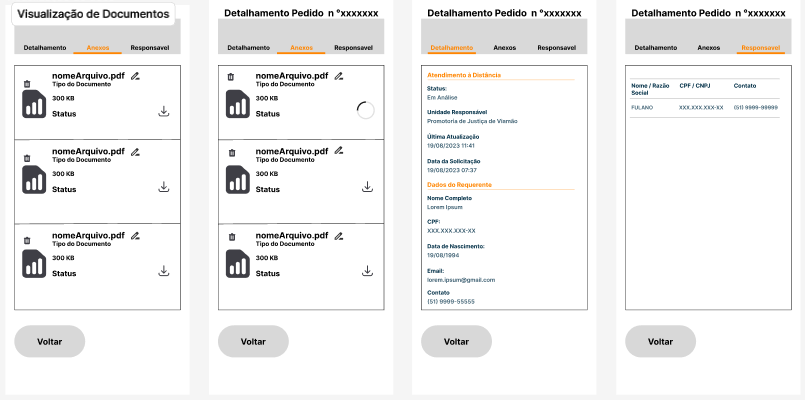
\includegraphics[width=1\linewidth]{conteudo//2 - ages I//conteudo//figures/figura7-resto-mais-mais-telas}
    Fonte: Figma do projeto
    \label{fig:mobile-visualization}
\end{figure}

Ao longo da implementação o projeto, realizou-se um style-guide a fim de
padronizar as telas e aprimorar a experiência do usuário. A Figura 8 apresenta
estas novas e últimas versões do aplicativo mobile.

\begin{figure}[H]
    \centering
    \small
    \caption{Telas finais mobile de boas-vidas, login, cadastro e home do projeto Vítimas de Crime}
    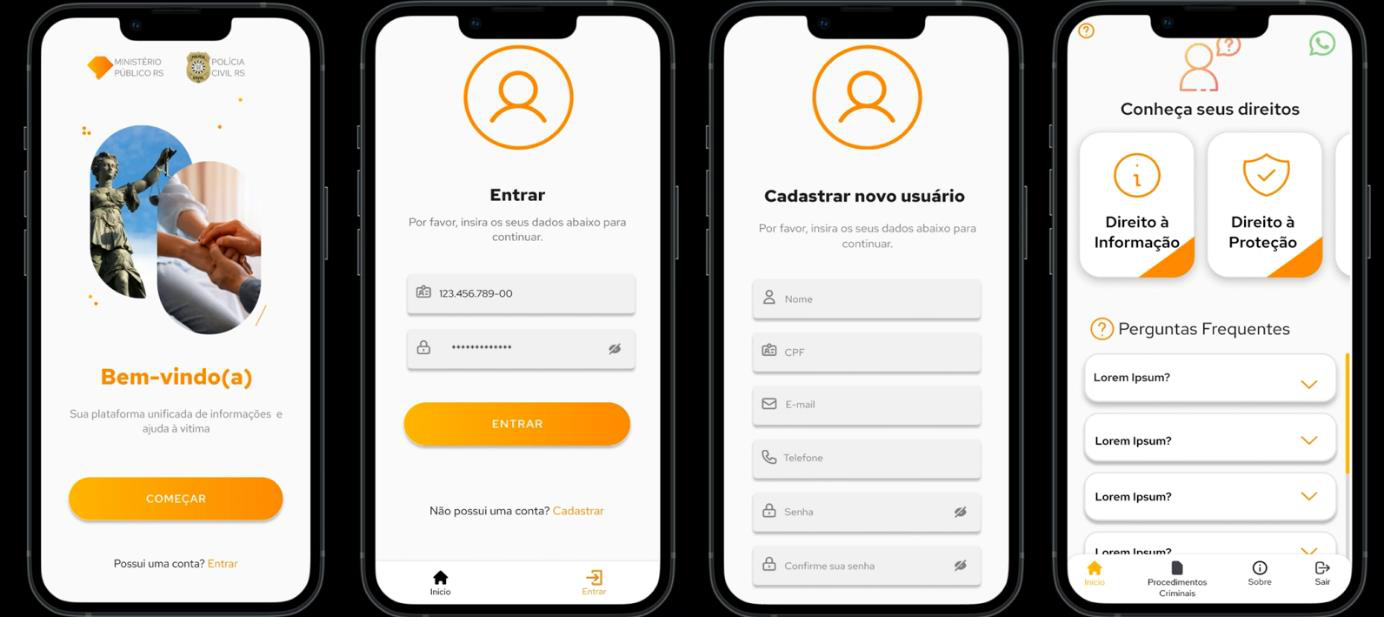
\includegraphics[width=1\linewidth]{conteudo//2 - ages I//conteudo//figures/figura8-telas-finais}
    Fonte: \textit{Wiki} do projeto
    \label{fig:final-mobile}
\end{figure}

Logo quando o aplicativo \textit{mobile} estava quase pronto, o time passou a desenvolver
as telas do \textit{website}. São apresentadas estas telas entregues nas Figuras 9 até 12.

\begin{figure}[H]
    \centering
    \small
    \caption{Tela web de boas-vidas do projeto Vítimas de Crime}
    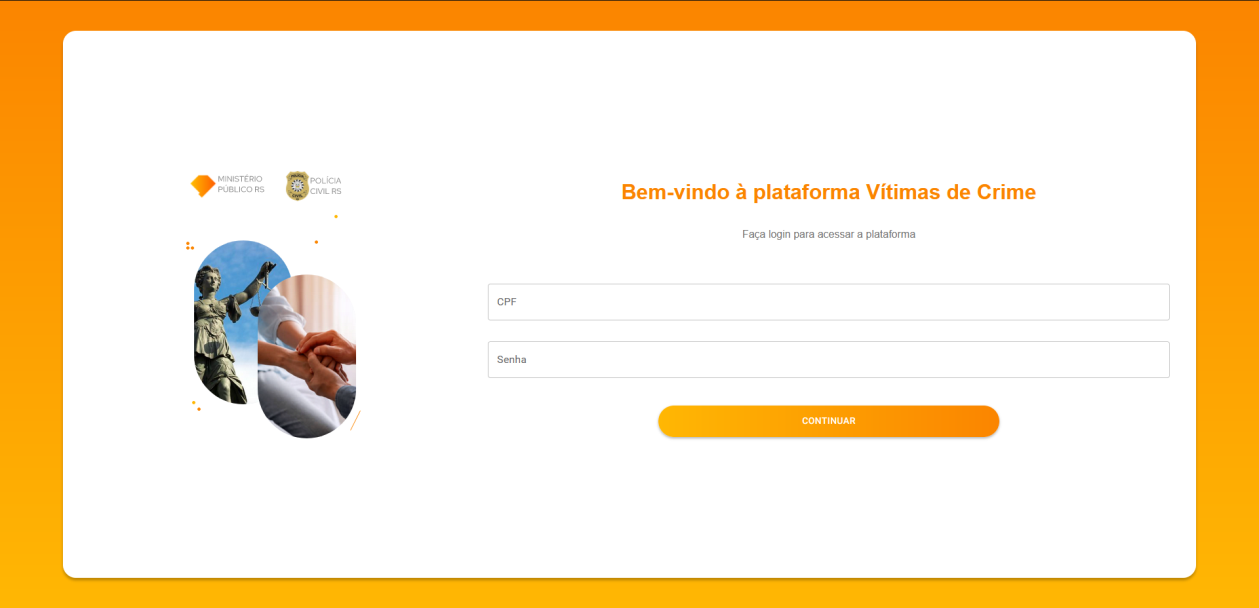
\includegraphics[width=1\linewidth]{conteudo//2 - ages I//conteudo//figures/figura9-web-tela-welcome}
    Fonte: Autor
    \label{fig:web-landing}
\end{figure}

\begin{figure}[H]
    \centering
    \small
    \caption{Tela web de procedimentos do projeto Vítimas de Crime}
    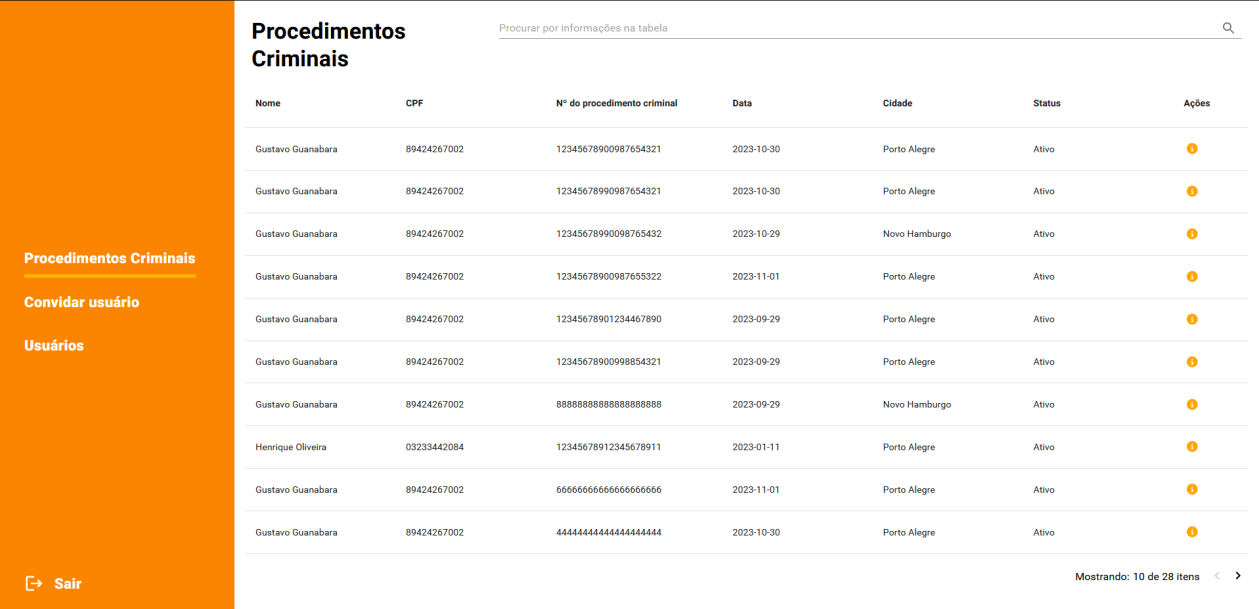
\includegraphics[width=1\linewidth]{conteudo//2 - ages I//conteudo//figures/figura10-web-tela-mais}
    Fonte: Autor
    \label{fig:web-procedures}
\end{figure}

\begin{figure}[H]
    \centering
    \small
    \caption{Tela web de convidar usuários do projeto Vítimas de Crime}
    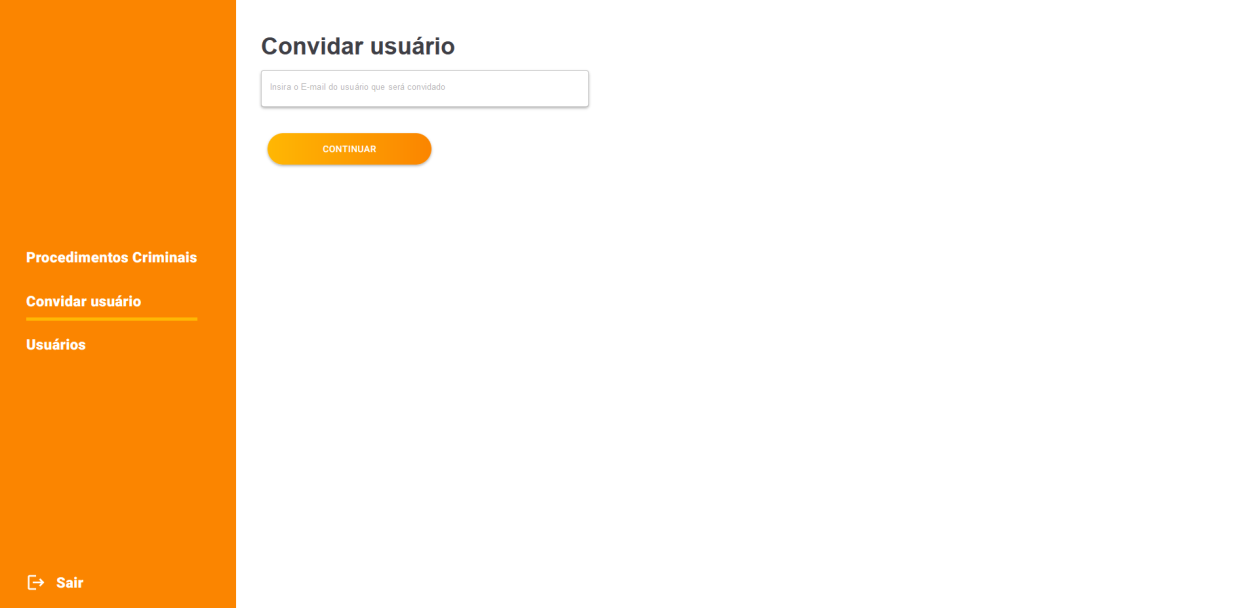
\includegraphics[width=1\linewidth]{conteudo//2 - ages I//conteudo//figures/figura11-tela-web-siuuu}
    Fonte: Autor
    \label{fig:web-invite}
\end{figure}

\begin{figure}[H]
    \centering
    \small
    \caption{Tela web de usuários do projeto Vítimas de Crime}
    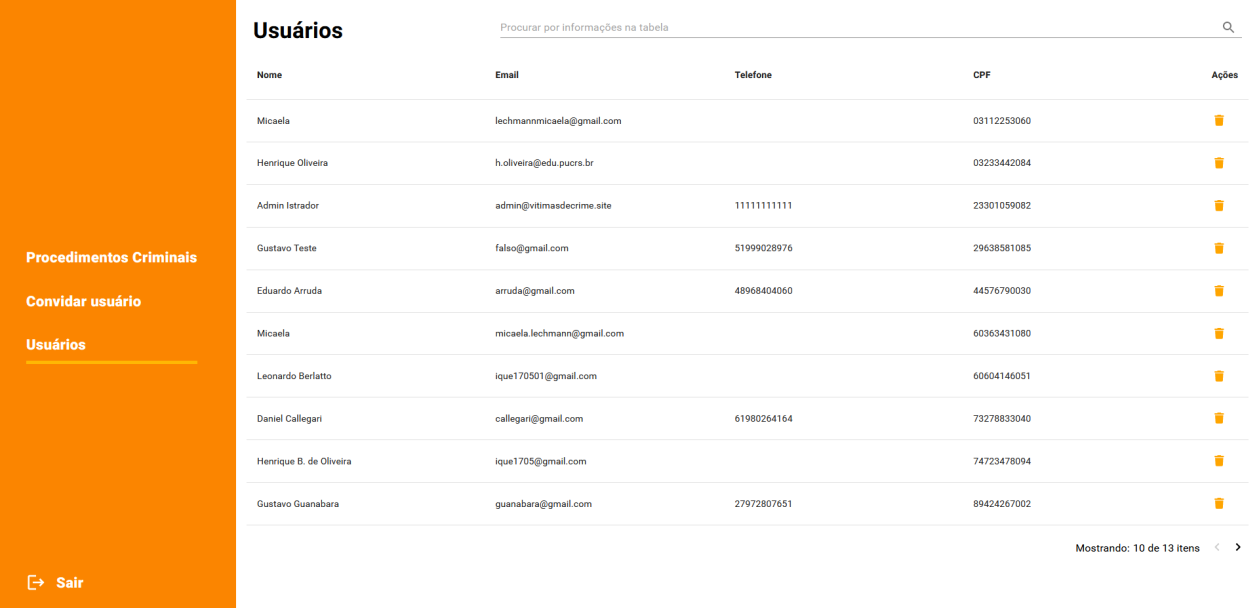
\includegraphics[width=1\linewidth]{conteudo//2 - ages I//conteudo//figures/figura12-tela-web-table}
    Fonte: Autor
    \label{fig:web-table}
\end{figure}

\subsection{Tecnologias Utilizadas}
  A implementação das APIs da aplicação e a gestão da autenticação no \textit{backend}
do projeto foram realizadas com a linguagem Kotlin, usando o framework Spring Boot,
Gradle como gerenciador de dependências e Selenium para testes de sistema. A
autenticação é gerenciada pela plataforma Keycloak, que implementa o protocolo
OAuth 2.

Além disso, foram utilizados recursos da AWS, incluindo S3 storage e EKS, e
para facilitar a configuração em diferentes ambientes e melhorar a escalabilidade
optamos pelo uso de containers Docker. Quanto ao \textit{frontend}, TypeScript foi escolhido
como a linguagem de principal, juntamente com React Native e Expo para o
desenvolvimento \textit{mobile}, enquanto React JS sendo utilizado para \textit{web}. \textit{Temp ref:
https://tools.ages.pucrs.br/vitimas-de-crime/wiki/-/wikis/Arquitetura do Projeto.}

\section[Atividades Desempenhadas Pelo Aluno no Projeto]{Atividades Desempenhadas Pelo Aluno no Projeto}

O intuito desta seção é fornecer uma explicação das tarefas desempenhadas
pelo aluno durante o desenvolvimento do projeto. As atividades e o uso das
tecnologias são categorizados em sprints, os quais representam intervalos de tempo
com metas e entregas específicas.

\subsection{Sprint 0}

O projeto tecnicamente teria iniciado após a primeira reunião com as
stakeholders do MP, que apresentaram sua proposta sobre um aplicativo de ajuda a
vítimas de crime. Porém, devido a possível confusão pelas duas partes (nossa e do
cliente), não foi possível determinar os requisitos e nem o escopo do projeto.

Tendo em vista este pequeno atraso, os AGES IV do projeto marcaram outra
reunião na mesma semana para definir de fato o que nos faltava para iniciar os
trabalhos. Após esta segunda reunião as primeiras tarefas já foram divididas, entre
escolha de tecnologias e a arquitetura para os AGES III, um quadro \textit{kanban} para
organizar as tasks e o design de mockups no figma das telas do app para os AGES I
e II.

Como AGES I e sem conhecimento de nenhuma tecnologia usada no projeto,
nesta \textit{sprint} acabei apenas observando e estudando o que teríamos que utilizar para
realização do produto. Em conjunto com outros AGES I desenvolvi algumas telas no
figma, porém meu foco foi maior em estudar o framework Spring Boot para o \textit{backend}
e React Native para o \textit{frontend}
\\
\\
\fbox{%
    \parbox{1\linewidth}{%
        \setlength{\parindent}{15pt}
            \itshape Minha experiência inicial de AGES I deixou muitíssimo a desejar. A não ser que o aluno em sua
            primeira AGES já  tenha trabalhado na área, é de extrema dificuldade que ele
            consiga exercer alguma função dentro do projeto.
    
            Há várias tecnologias que não são abordadas em nenhuma disciplina
            específica, e, em grande parte, espera-se que o aluno já tenha conhecimento e/ou
            experiência em seu uso. A meu ver isso tudo impacta para uma vivência que não
            agrega muito no currículo dos alunos.
    
            Não foi de ajuda também, o fato que o início do projeto atrasou pela confusão
            das clientes, além da cultura forte de herói no time.
    }%
}

\subsection{Sprint 1}

Tendo o escopo inicial pronto, as primeiras tasks foram definidas e divididas
(geralmente em duplas para facilitar com os AGES I) entre o time. Nesta sprint fiquei
inicialmente encarregado com uma task do backend, especificamente a implementação do login na parte de
autenticação do app.

Boa parte deste tempo acabei estudando e tentando entender o que devia ser
feito na minha task, devido a minha falta de conhecimento com as tecnologias
envolvidas. Como acabei pedindo ajuda muito tarde, dois colegas (Gabriel Lima e
Leonardo Berlatto, AGES II e III respectivamente) acabaram me auxiliando e me
mostrando o que deveria ser feito.
    
A primeira entrega para as stakeholders acabou sendo atrasada, e
consequentemente a task que eu estava envolvido. O AGES III que estava me
ajudando acabou terminando a atividade sozinho.
\\

\fbox{%
    \parbox{0.95\linewidth}{%
        \setlength{\parindent}{15pt}
            \itshape A maior lição que aprendi nesta sprint foi de pedir ajuda o mais cedo possível,
    acabei me sentindo culpado por atrasar o time com minha teimosia e timidez. Por
    mais que sou crítico da disciplina de AGES I, meus colegas do time sempre me
    ajudaram e eram extremamente prestativos. Eu não só poderia como deveria ter me
    expressado muito antes, e talvez assim, conseguiria ter feito mais pelo projeto.
    }%
}
\subsection{Sprint 2}

Durante esta etapa do projeto acabei participando diretamente no frontend do
aplicativo mobile ao invés do backend. Tendo isso em mente, foquei mais no estudo
do framework específico ao invés das tecnologias do projeto como um todo.

Trabalhei junto com o AGES I Gustavo Pretto que me auxiliou bastante
especificamente na criação de componentes e desenvolvimento de telas. No final,
tanto por trabalhos ou provas de outras disciplinas e por dificuldades do time, a
entrega desta sprint foi muito incompleta.
\\

\fbox{%
    \parbox{0.95\linewidth}{%
        \setlength{\parindent}{15pt}
            \itshape    A sprint 2 foi imensamente difícil, o período coincidiu com diversas atividades
    acumuladas e em datas próximas de outras cadeiras. Não só isso, mas também o
    fato que minha reunião one-on-one foi onde tive que encarar a realidade que não
    estava contribuindo para o time.
    
        Eu estava perdido no ambiente do grupo, tanto quanto nos estudos das
    tecnologias novas que nunca havia visto. Tentei bastante virar a chave nesta sprint,
    mas acho que algumas ideias do time e mentalidade de alguns não foram de muita
    ajuda também. A técnica de pair-programming foi utilizada para servir de ajuda aos
    iniciantes e agilizar o processo, tendo em vista que a entrega na sprint 1 foi
    incompleta.
    
        Minha dupla funcionou bem, mas outras que talvez precisassem de mais ajuda
    acabavam sendo um pouco teimosos para aceitar ajuda. Quando terminávamos
    alguma task e não havia outra imediatamente para trabalharmos, nossa dupla
    acabava ficando ociosa devido a esse problema. Talvez com um pouco mais de
    insistência minha, e outros com menos teimosia, poderíamos ter feito uma entrega
    melhor para o cliente.
    }%
}
\subsection{Sprint 3}

O dia da entrega da sprint passada contou com talvez metade do time presente,
e com uma entrega dita pelos AGES IV do projeto como a “\textit{pior entrega que já viram
em um projeto da AGES}”. Ao invés da retrospectiva, foi decidido realizar uma reunião
de emergência pelos presentes para conversar sobre o que estava acontecendo, o
que devia mudar e talvez como proceder.

Feita a reunião e todos tendo dito suas opiniões, o time resolveu abandonar
certas ideias do \textit{agile} visto que a rotina de trabalho não estava fluindo como esperado.
Os AGES IV tomaram uma medida mais direta na atribuição de duplas e tasks, tendo
maior controle sobre o projeto em si.

Continuei no \textit{frontend} esta sprint e de dupla com o AGES II Otávio Cunha.
Fomos encarregados de resolver algumas dívidas técnicas como responsividade na
tela de cadastro do usuário e alguns componentes, além de desenvolver novas telas
sobre visualização de documentos em procedimentos criminais.

Acabamos mexendo bastante especificamente em CSS para resolver as
dívidas de responsividade, já na parte de visualização de documentos conseguimos
trabalhar mais tranquilamente. O que mais nos tomou tempo foi integrar corretamente
as rotas do backend para chamar os documentos de cada procedimento.

Mesmo com estas mudanças a entrega ainda assim precisou de ajustes de
última hora dos AGES III e IV, devido a falta de testes pelo time na hora de integrar
as suas tarefas.
\\

\fbox{%
    \parbox{0.95\linewidth}{%
        \setlength{\parindent}{15pt}
            \itshape    A reunião do dia da entrega realmente foi quando o time virou a chave, após
                este dia todo pareciam mais envolvidos com o projeto tanto quanto nas reuniões
                diárias e nos canais de comunicação. Aqui  também, percebi bastante meu
                melhor desempenho e atitude.
                
                Todavia, mesmo com as melhorias aparentes a entrega constou com
                mudanças locais pelos AGES IV. Notei que alguns AGES I e II ainda pecavam na
                hora de testar cada uma de suas tarefas com o projeto todo.
    }%
}
\subsection{Sprint 4}

Na sprint final segui trabalhando nos toques finais na tela de anexo integrando
alguns componentes finais necessários, e tentei desenvolver a lógica de download de
arquivo do componente documento. Esta funcionalidade de download acabou
provando ser trabalhosa e complexa demais, tomando muito tempo com pouco
progresso. Sendo assim minha dupla foi realocada para refatorar a tela de home do
aplicativo.

Após a tela de home estar pronta fui designado a parte web do
nosso projeto. Acabei ajudando o desenvolvimento da tela de listagem dos
procedimentos criminais, de novo com o colega Gustavo Pretto, na maior parte do
tempo arrumando a integração com as rotas do backend e junto com o próprio
ambiente que estava cheio de erros.
\\
\\
\fbox{%
    \parbox{1\linewidth}{%
        \setlength{\parindent}{15pt}
            \itshape    A última sprint foi relativamente tranquila quando comparada ao
que aconteceu previamente no projeto. A atitude do time já tinha mudado a esse
ponto e senti que maioria do pessoal conseguia trabalhar e/ou pedir ajuda no que era necessário.
Os últimos dois finais de semanas contaram com o time cooperando para sanar
alguns detalhes finais.

Claro que se eu pudesse recomeçar este projeto do zero, eu iria
aproveitá-lo melhor, eu poderia ter tomado a iniciativa anteriormente, comunicado
mais e coisas do tipo. Porém, por mais que a primeira metade deste projeto tenha sido
um tanto quanto desafiadora e intimidante, acho que serviu muito bem como lição e
aprendizado para minhas futuras AGES
    }%
}
\section[Conclusão]{Conclusão}

Tanto pela minha limitada experiência com as tecnologias
abordadas, quanto pela minha estreia na AGES, este projeto acabou sendo
incrivelmente intimidador e desafiador. Minha timidez e receio de não conseguir
realizar algumas tarefas também contribuíram para a dificuldade.

Certamente, se eu tivesse abordado esse problema no início do semestre,
poderia ter ajudado o time de forma mais eficaz. Acho também que alguns colegas
sofreram da mesma timidez pois sempre houve um problema de muito silêncio por
parte dos AGES I e alguns II. O que acabou sendo uma pena, ainda mais quando
muitos do time incluindo os AGES II, III e IV sempre foram de muita ajuda e
comprometidos com o projeto.

Além dos desafios internos enfrentados pela equipe, tivemos problemas já na
sprint 0 ao tentar levantar os requisitos das stakeholders e definir o escopo do projeto.
Devido à falta de clareza sobre o propósito da primeira reunião, não conseguimos
levantar nenhum requisito nesse dia, resultando em um atraso de uma semana no
início do desenvolvimento. Adicionalmente, o escopo, que foi delineado após a
reunião, mostrou-se extremamente aberto e sujeito a mudanças durante novos
encontros com os clientes.

Dito as dificuldades e problemas, por mais que fui crítico com a disciplina de
AGES I e que este projeto em específico provou ser confuso e complexo, aprendi
muito com meus colegas. Afinal, a superação de desafios é
essencial ao avanço e desenvolvimento, pois é na presença de obstáculos que
encontramos a oportunidade de progredir.

De lição levo comigo que a comunicação é um dos aspectos de maior
relevância do trabalho em grupo. Por mais que foram escolhidas tecnologias
complexas e avançadas, os problemas vistos no projeto em termos de dificuldade
teriam sido sanados e resolvidos rapidamente caso a comunicação do time fosse
melhor.

Para minha reflexão final, noto que aprimorei minhas habilidades de interagir e
me expressar com meus colegas referente ao espaço de trabalho. Tenho certeza de
que para minhas futuras AGES estes pontos serão de extrema importância.